\chapter{Εισαγωγη}

\section{Γενικά}

Στην σύγχρονη κοινωνία παρουσιάζεται εκθετική αύξηση της συλλογής δεδομένων, καθως η υπολογιστική τεχνολογία, η δικτυακή συνδεσιμότητα και ο ψηφιακός χώρος αποθήκευσης γίνονται συνεχώς πιό προσιτά. Κάθε δευτερόλεπτο, εκατομμύρια καταχωρήσεις απο οργανισμούς, ετaιρίες και μέσα κοινωνικής δικτύωσης, έχουν οδηγήσει σε εκτίναξη
την παραγωγή δεδομένων σε 3 πεντάκις εκατομμύρια \textlatin{bytes} ημερισίως. Χαρακτηριστικό είναι ότι μόνο η \textlatin{google} στεγάζει περισσοτερα από 10 \textlatin{exabytes} δεδομένων.

Για κάθε άνθρωπο, από την στιγμή της γέννησής του, υπάρχει τουλάχιστον μια καταχώρηση σε μια συλλογή δεδομένων. Σε διάφορους τομείς, από ιδιωτικούς και κοινωνικούς φορείς όπως τράπεζες, νοσοκομεία, τηλεφωνικούς παρόχους, ακόμα και επιχειρήσεις, συλλέγονται και αποθηκεύονται αναλυτικά προσωπικές πληροφορίες των πελατών τους. Είναι γεγονός ότι όσο περισσότερες πληροφορίες υπάρχουν για κάποιον στις βάσεις δεδομένων εταιριών και οργανισμών, τόσο καλύτερες υπηρεσίες παρέχονται στο άτομο αυτό, αλλά και αντίστροφα, επωφελούνται οι αναλυτές των βάσεων δουλεύοντας με καλύτερο/μεγαλύτερο δείγμα: Στατιστικά δεδομένα υγείας για ένα άτομο που συλλέγονται είτε από τους άμεσα εμπλεκόμενους φορείς, είτε έμμεσα απο μικροσυσκευές (\textlatin{smartwatches, smartphones},κλπ) μπορούν να βοηθήσουν στην πρόληψη μιας σοβαρής ασθένιας, μικροδεδομένα μετακινήσης από τους κατοίκους μιας πόλης συμβάλουν στην βελτίωση της κυκλοφορίας, ενώ ανάλυση σε βάσεις δεδομένων εγκληματιών οδηγεί σε πιθανή εξιχνίαση κάποιας υπόθεσης. 

\subsection{Ανάγκη για προστασία των δεδομένων}

Η αποκάλυψη προσωπικών στοιχείων και προτιμήσεων είναι, θα τολμούσαμε να πούμε, αναγκαία για την ομαλότερη και αποτελεσματικότερη λειτουργία εφαρμογών και υπηρεσιών. Η συνεχής αύξηση όμως της συλλογής δεδομένων οδηγεί σε υπερβολική συγκέντρωση ατομικών πληροφοριών. Χαρακτηριστικό είναι ότι περισσότερες από 15.000 ειδικευμένες βάσεις περιέχουν δυο δισεκατομμύρια ονόματα καταναλωτών μαζί με μεγάλο όγκο προσωπικών πληροφοριών, ενω ο μέσος καταναλωτής βρίσκεται καταχωρημένος τουλάχιστον σε 25 διαφημιστικές λίστες. Πολλές από αυτές τις λίστες, αφού οργανωθούν σύμφωνα με γνωρίσματα όπως εισόδημα, ηλικία, πολιτικές και θρησκευτικές απόψεις, αγοράζονται και πωλούνται καθημερινά. Η κατάχρηση συνεπώς των βάσεων δεδομένων είναι αναπόφευκτη.

Οι κάτοχοι των συνόλων δεδομένων συνήθως δίνουν εγγύηση ότι οι καταχωρήσεις τους είναι ασφαλείς, όμως πολλές είναι οι περιπτώσεις που χρησιμοποίήθηκαν βάσεις δεδομένων για παραβίαση της ιδιωτικότητας κάποιου ατόμου. Αξίζει να αναφέρουμε τους λόγους:
\begin{itemize}
\item Εξαπάτηση
\item Στρατηγικές ενέργειες
\item Σφάλματα
\end{itemize}
Προκύπτει λοιπόν η ανάγκη για αυστηρότερη προστασία της ιδιωτικότητας των πληροφοριών.

Εντυπωσιακό είναι το αποτελέσμα μιας πρόσφατης δημοσκόπησης (\textlatin{YouGov,2017}) που ανεφέρει ότι το 1/5 των κατοίκων του Ηνωμένου Βασιλείου ανησυχούν για την πώληση των προσωπικών τους δεδομένων σε άλλες εταιρίες, ενώ το 12\% ανησυχεί οτί τα ήδη καταχωρημένα δεδομένα τους μπορεί να υποκλαπούν. Αν αναλογιστούμε ότι τα ποσοστά αυτά αντιστοιχούν σε εκατομμύρια πολιτών, συμπεραίνουμε ότι η απαίτηση για ασφάλεια στις συλλογές δεδομένων, τόσο από την μεριά των διαχειριστών όσο και των υποκειμένων, είναι ολοένα και μεγαλύτερη. 

Αυτό, δεν αφήνει ασυγκίνητες ούτε τις κυβερνήσεις ανά τον κόσμο, τοποθετώντας την προστασία των δεδομένων ψηλά στην ατζέντα τους. Η Ευρωπαική Ένωση ψήφισε πρόσφατα το \textlatin{GDPR - General Data Protection Regulation} -με ημερομηνία εφαρμογής τον Μάη του 2018- έναν κανονισμό πρώτον για την προστασία των φυσικών προσώπων έναντι της επεξεργασίας των προσωπικών δεδομένων τους και δεύτερον για την ελεύθερη διακίνηση αυτών.

Η προστασία της ιδιωτικότητας είναι αδιαμφισβήτητα μια ανάγκη της εποχής, καθώς η συλλογή δεδομένων αυξάνεται με γεωμετρική πρόοδο. Το μεγάλο ζήτημα είναι η παροχή των απαραίτητων πληροφοριών και η ορθή χρήση τους απο τρίτους, αποφεύγοντας ταυτόχρονα οποιαδήποτε παραβίαση. Με το πέρασμα των χρόνων έχουν διατυπωθεί ποικίλες μέθοδοι και τεχνικές προστασίας της ιδιωτικότητας των ευαίσθητων δεδομένων με σκοπό την διατήρηση της ισορροπίας ανάμεσα στην εκμετάλλευση των προσωπικών δεδομένων και τον σεβασμό προς τα άτομα.


%{Ως αποτέλεσμα όλο και περισσότερα σύνολα δεδομένων δημοσιοποιούνται, είτε ως αποτέλεσμα κυβερνητικών αποφάσεων, είτε ως δείγμα προς εξόρυξη. 
%Συχνά εντός των δεδομένων αυτών εμπεριέχονται προσωπικές πληροφορίες όπως οικονομική κατάσταση, ιατρικό ιστορικό, πολιτικές πεποιθήσεις, οι οποίες δεν είναι επιυθμητό να διαρρεύσουν. 

\subsection{Παροχή ασφάλειας}

Ο έλεγχος πρόσβασης (\textlatin{access control}) στην εκάστοτε βάση, χρησιμοποιώντας κλασικές μεθόδους κρυπτογράφισης, αποτελεί την καθολική τεχνική προστασίας των δεδομένων. Αυτό δυστυχώς δεν εφαρμόζεται πάντα, αφού συνήθως τα σύνολα δεδομένων προς ανάλυση είναι δημοσίως διαθέσιμα. Η μέθοδος αυτή είναι χρήσιμη μόνο αν εφαρμοστεί ορθόδοξα, ώστε να αποτρέπει την πρόσβαση στα δεδομένα σε οποιονδήποτε επιτιθέμενο αλλά εμφανίζοντας όλη τη βάση στον καλόβουλο αναλυτή. Η μελέτη της μεθόδου αυτής ωστόσο ξεφεύγει από τα όρια της εργασίας μας.

Η παραδοσιακή προσέγγιση του προβλήματος της προστασίας των εγγραφών είναι η «ανωνυμοποίηση» του συνόλου δεδομένων αποκρύπτοντας ή κρυπτογραφώντας χαρακτηριστικά τα οποία θα μπορούσαν να αποκαλύψουν την ταυτότητα ενός ατόμου, όπως όνομα, διεύθυνση, ημερομηνία γέννησης. Ως αποτέλεσμα, προβάλλεται μια «εξυγιασμένη»\textlatin{(sanitized)} βάση δεδομένων. Παρ' όλ' αυτά, αποδεικνύεται ότι η απλή απόκρυψη πληροφορίας δεν είναι αρκετή, διότι σε συνδιασμό με κατάλληλη βοηθητική γνώση είναι δυνατόν να αποκαλυφθεί η ταυτότητα ενός υποκειμένου.

Κατά καιρούς, έχουν γίνει προσπάθειες για την μεγιστοποίηση της ασφάλειας βελτιώνοντας τις τεχνικές ανωνυμοποίησης. Οι περισσότερες τεχνικές χρησιμοποιούν καποιά μορφή μετασχηματισμού των δεδομένων, με στόχο την γενίκευση/ομαδοποίηση των πληροφοριών ώστε να διασφαλιστεί η ιδιωτικότητα. Παρακάτω θα αναφέρουμε τις κυριότερες από αυτές, τις οποίες θα παρουσιάσουμε αναλυτικά στα επόμενα κεφάλαια.
\begin{itemize}
\item \textlatin{k-anonymity}: Το μοντέλο αυτό μειώνει την διακριτικότητα των πληροφοριών με χρήση της τεχνικής της γενίκευσης, εξασφαλίζοντας ότι ο επιτιθέμενος δεν καταφέρνει να προσδιορίσει μοναδικά κάποια εγγραφή σε μια βάση δεδομένων αφού θα υπάρχουν τουλάχιστον $k-1$ εγγραφές με ίδια ακριβώς χαρακτηριστικά. 
\item \textlatin{l-diversity, t-closeness}: Τα μοντέλα αυτά σχεδιάστηκαν για να διαχειριστούν τις αδυναμίες της μεθόδου της \textlatin{k-anonymity}, η οποία είναι ανεπαρκής στο να προστατέψει από την αποκάλυψη τιμών γνωρισμάτων των εγγραφών. Η \textlatin{l-diversity} το αποτρέπει αυτο ομαδοποιώντας τις καταχωρήσεις σε κλάσεις με $l$ τουλάχιστον διαφορετικές τιμές απο κάθε χαρακτηριστικό. Η \textlatin{t-closeness} πάει ένα βήμα παραπέρα, ορίζοντας συγκεκριμένο κατώφλι για την διαφορά της κατανομής ενός χαρακτηριστικού σε μια κλάση απο την κατανομή σε όλη την βάση.
\end{itemize}


Ένας άλλος τρόπος προσέγγισης του προβλήματος είναι η τυχαιοποίηση, στην οποία δεν δημιουργείται μια νέα εξυγιασμένη βάση όπως στις παραπάνω μεθόδους, αλλά παρέχεται ιδιωτικότητα μέσω της προσθήκης θορύβου στα δεδομένα. Ο κύριος εκφραστής της διαδραστικής μεθόδου είναι η Διαφορική Ιδιωτικότητα.

 Η τεχνική αυτή δεν στηρίζεται στον διαχωρισμό της βάσης δεδομένων σε υποσύνολα όπως οι προαναφερθείσες, αλλά έχει ως σκοπό τον περορισμό της βαρύτητας των δεδομένων στα αποτελέσματα που εξορύσσονται απο την βάση.


Όπως είδαμε, η ιδιωτικότητα σε μια βάση μπορεί να επιτευχθεί με διάφορους τρόπους. Παρακάτω ταξινομούμε τα είδη προστασίας που μπορούν να εφαρμοστούν σε διάφορα επίπεδα της ροής πληροφοριών κατά την ανάλυση δεδομένων.



\subsection{Ροή πληροφοριών}

Η παρακάτω προσέγγιση δείχνει την ροή πληροφορίας ξεκινώντας από τις προσωπικές πληροφορίες ενός ατόμου και καταλήγοντας στον αναλυτή. Τα δεδομένα συλλέγονται σε μια βάση που την ελέγχει ένας διαχειριστής. Το επιθυμητό είναι οι αναλυτές να μπορούν να πραγματοποιούν επερωτήσεις και υπολογισμούς σε αυτήν ώστε να συλλέξουν στατιστικά στοιχεία, ενώ ένας επιτιθέμενος να μην μπορεί να εξάγει ευαίσθητα δεδομένα για συγκεκριμένα άτομα.

Για να προστατευτεί η ιδιωτικότητα των ατόμων αυτών πρέπει να υπάρχει έλεγχος της ροής πληροφοριών κατά την διαδρομή τους από το ένα άκρο στο άλλο \textlatin{\cite{hay}}


\begin{figure}[h!]
  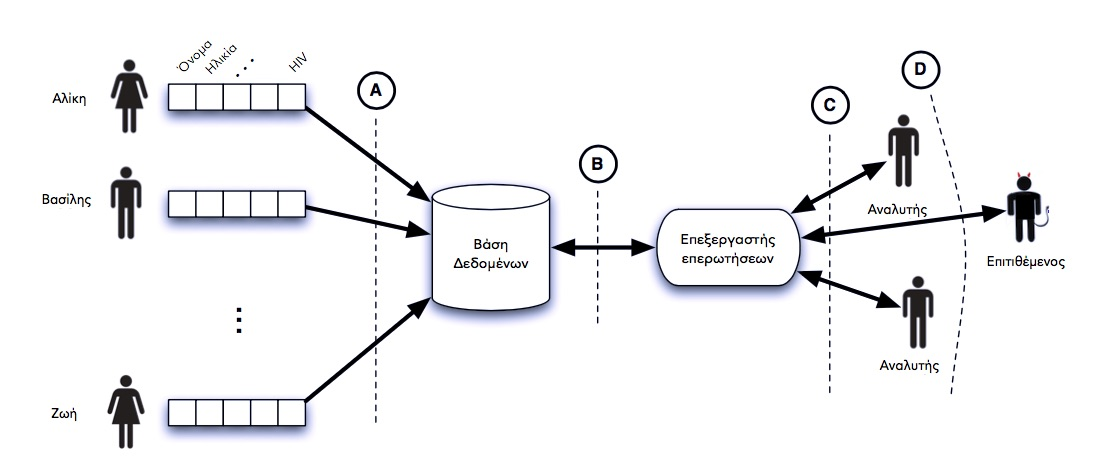
\includegraphics[width=\linewidth]{images/Hay.jpg}
  \caption{Στάδια ελέγχου ροής πληροφοριών}
  %\label{fig:boat1}
\end{figure}


Α. Διαταραχή εισόδου: Τα ίδια τα άτομα μπορούν να αλλοιώσουν τα δεδομένα που δίνουν στη βάση, προσθέτοντας θόρυβο. Με αυτόν τον τρόπο ο επιτιθέμενος δεν θα είναι ποτέ σίγουρος οτι οι ευαίσθητες πληροφορίες για κάποιο άτομο είναι σωστές, ενώ τα στατιστικά που συγκεντρώνουν οι αναλυτές δεν υφίστανται αξιόλογη μεταβολή.

Β. Μετασχηματισμός δεδομένων: Η αρχική βάση δεδομένων αναδομείται σε μια νέα εξυγιασμένη βάση στην οποία οι ευάισθητες πληροφορίες για συγκεκριμένα άτομα δεν είναι πια διακριτές. Σε αυτό το επίπεδο εφαρμόζεται το μοντέλο της \textlatin{k-anonymity}.

\textlatin{C}. Διαταραχή απάντησης επερωτήσεων: Οι αναλυτές μπορούν να επεξεργαστούν τα δεδομένα αλλά για να διασφαλιστεί η ιδιωτικότητα έχει προστεθέι θόρυβος. Εδώ εφαρμόζεται το μοντέλο της Διαφορικής Ιδιωτικότητας.

\textlatin{D}. Έλεγχος Πρόσβασης: Η βάση δεν είναι δημοσίως διαθέσιμη και μόνο οι έμπιστοι ερευνητές έχουν πρόσβαση. Έτσι αποτρέπεται η διαρροή ευαίσθητων δεδομένων σε κακόβουλα άτομα.





\subsection{Διατήρηση ποιότητας}

Όπως είναι προφανές, η απόκρυψη και η γενίκευση των δεδομένων έχει ως αποτέλεσμα την αλλοίωση της πληροφορίας και την απώλεια της αποτελεσματικότητας. Είναι γεγονός ότι το ποσό ανωνυμίας που έχει μια βάση δεδομένων είναι αντιστρόφως ανάλογο με την ποιότητα:

Η δημοσίευση της βάσης δεδομένων στο ακέραιο παρέχει την καλύτερη ποιότητα, ενώ η πλήρης απόκρυψη την καλύτερη ιδιωτικότητα. \textlatin{\cite{Sweeney:2001:CDC:935675}}
\begin{center}
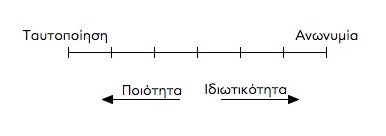
\includegraphics[scale=0.6]{images/Tension.jpg}
\end{center}
Κανένα από τα δυο άκρα δεν είναι επιθυμητό να προσεγγίζεται απο ένα σύνολο δεδομένων. Αφενός διότι στο ένα δεν θα παρέχεται καμία ασφάλεια στις εγγραφές και αφετέρου διότι στο άλλο τα δεδομένα θα είναι τόσο διαταραγμένα, που η ανάλυση θα είναι αδύνατη. Στο πλαίσιο της εργασίας αυτής θα συγκρίνουμε στο δυνατόν τις τεχνικές ιδιωτικότητας ως προς την ισορροπία που διατηρούν μεταξύ της προστασίας των εγγραφών και της τελικής ποιότητας των δεδομένων που παρέχονται στον αναλυτή. 


\section{Σκοπός}

Η παρούσα διπλωματική εργασία έχει τους εξής στόχους:
\begin{itemize}
\item Παρουσίαση τεχνικών και μεθοδολογιών που χρησιμοποιούνται για την ενίσχυση της ιδιωτικότητας στις βάσεις δεδομένων.
\item Επισκόπηση και κριτική αξιολόγηση από την σκοπιά της ασφάλειας και ιδιωτικότητας των υπό εξέταση προτάσεων/μεθοδολογιών.
\item Ανάδειξη κρίσιμων και ανοικτών ζητημάτων, καθώς και κατάδειξη προοπτικών για περαιτέρω έρευνα.
\end{itemize}


\section{Δομή Εργασίας}

Η εργασία είναι δομημένη ως εξής:

Στο δεύτερο κεφάλαιο παρουσιάζονται τα βασικά στοιχεία του προβλήματος. Γίνεται παρουσίαση και ανάλυση της μεθόδου \textlatin{k}-ανωνυμία 
(\textlatin{k-anonymity}). 
Δίνονται παραδείγματα και εξετάζονται οι αδυναμίες που την χαρακτηρίζουν. Στη συνέχεια, παρουσιάζονται δυο τεχνικές βελτιστοποίησης της μεθόδου της $k$-ανωνυμίας , η $l$-διαφορετικότητα (\textlatin{l-diversity}) και η $t$-εγγύτητα (\textlatin{t-closeness}). Αναλύεται η δυνατότητα και το κόστος εφαρμογής τους και εξετάζονται τα μειονεκτήματα χρήσης τους.

Στο τρίτο κεφάλαιο γίνεται θεμελίωση και ανάλυση του μοντέλου της Διαφορικής Ιδιωτικότητας. Δίνονται παραδείγματα, αναλύεται η επίδοσή των μηχανισμών και εξετάζεται η χρησιμότητα τους. 

Στο τέταρτο κεφάλαιο περιγράφονται αλγόριθμοι ανωνυμοποίησης που χρησιμοποιούν κυρίως τις τεχνικές γενίκευσης από το δεύτερο κεφάλαιο.

Στο πέμπτο κεφάλαιο αναπτύσσονται αλγοριθμικές εφαρμογές που υλοποιούν τα μοντέλα της Διαφορικής Ιδιωτικότητας. 

Στο έκτο κεφάλαιο συνοψίζονται τα αποτελέσματα της διπλωματικής εργασίας, αναφέρονται πιθανά ανοιχτά ζητήματα  καθώς επίσης και η προοπτική για περαιτέρω έρευνα. 

\clearpage


\section{\textlatin{Ralated Work}}

\subsection{ \textlatin{Blockchain}}

Η τεχνολογία \textlatin{Blockchain} είναι ένα από τα δημοφιλέστερα ζητήματα των τελευταίων ετών και έχει ήδη αρχίσει να αλλάζει τον τρόπο ζωής της σύγχρονης κοινωνίας εξ' αιτίας της επιρρόης της σε επιχειρήσεις και βιομηχανίες. Παρ'όλο που η τεχνολογία αυτή είναι ευρέως γνωστό ότι παρέχει αξιόπιστες υπηρεσίες, τα θέματα ασφάλειας και οι προκλήσεις πίσω από αυτή την καινοτόμο μεθόδο είναι κάτι που δεν πρέπει να μας εφησυχάζει.

Το μοντέλο \textlatin{blockchain} δεν εκφράζει μια απλή τεχνική, αλλά έναν συνδιασμό κρυπτογραφικών, μαθηματικών, αλγορίθμικών και οικονομικών μεθόδων, πάνω σε \textlatin{peer-to-peer} δίκτυα, που στοχεύουν στην επίλυση παραδοσιακών κατανεμημένων προβλημάτων συγχρονισμού σε βάσεις δεδομένων. Τα βασικά στοιχεία που χαρακτηρίζουν το μοντέλο είναι η αποκέντρωση, λόγω της μη χρήσης  κεντρικών εξυπηρετητών, η διαφάνεια, το \textlatin{open source} λογισμικό, η αδυναμία μεταβολής των εγγραφών και η ανωνυμία.

Κάθε εγγραφή που δημιουργείται από έναν κόμβο σε ένα δίκτυο του μοντέλου \textlatin{blockchain}, αφού ελεγχθεί για την εγκυρότητα της, τοποθετείται σε ένα \textlatin{block} μαζί με άλλες εγγραφές. Κάθε \textlatin{block} επισφραγίζεται με ένα «\textlatin{Proof of Work}», υπολογισμένο από έναν από τους κόμβους του δικτύου μέσω μιας συνάρτησης κατακερματισμού η οποία συνδυάζει στοιχεία του τρέχοντος \textlatin{block} αλλά και του προηγουμένου. Στη συνέχεια συνδέεται στην «αλυσίδα». Με αυτόν τον τρόπο καθίσταται αδύνατη η παραβίαση κάποιου \textlatin{block}, εκτός αν οι επιτιθέμενοι κατέχουν την πλειοψηφία της υπολογιστικής ισχύς των κόμβων του δικτύου.

Πέραν αυτής της υποθετικής κατάστασης, γνωστή και ως «51\% \textlatin{attack}», που θα έβαζε σε κίνδυνο την αλυσίδα\textlatin{\cite{bastiaan2015preventing}}, πρόσφατες έρευνες έχουν αναδείξει αρκετά θέματα ασφάλειας στα \textlatin{blockchain}. Ένα από τα σημαντικότερα είναι το \textlatin{Hard/Soft Fork}, που περιγράφει την  εμφάνιση προβλημάτων από την μη ταυτόχρονη αναβάθμιση λογισμικού των κόμβων.

Δεν υπάρχει αμφιβολία ότι το μοντέλο \textlatin{blockchain} είναι ένα κρίσιμο θέμα της εποχής. Όσο το χρησιμοποιούμε και επωφελούμαστε των δυνατοτήτων του, τόσο πρέπει να επιφυλασόμαστε και να εξετάζουμε πιθανά θέματα ασφάλειας που θα προκύπτουν.


\subsection{\textlatin{Cloud Privacy}}

Οι υπηρεσίες νέφους έχουν μπει για τα καλά στη ζωή μας, αφού οι απαιτήσεις χώρου, χρόνου και ταχύτητας συνεχώς αυξάνονται. Πολλές εταιρίες Πληροφορικής και οργανισμοί προσφέρουν αλλά και χρησιμοποιούν εφαρμογές και υπηρεσίες νέφους, μια τεχνολογία η οποία κατα κύριο λόγο χρησιμοποιεί υπολογιστές και εξυπηρετητές ενός δικτύου για την μεταφορά, την επεγεργασία και την αποθήκευση των δεδομένων.

Όπως σε κάθε νέα τεχνολογία, έτσι και στο \textlatin{Cloud Computing} παρουσιάζονται αρκετά θέματα αφαλείας, ένα από τα σημαντικότερα είναι η προστασία των δεδομένων. Οι οργανισμοί δεν πρόκειται να μεταφέρουν τα δεδομένα τους σε απομακρυσμένους εξυπηρετητές αν δεν λάβουν εγγύηση για προστασία των δεδομένων από τους παρόχους υπηρεσιών νέφους. 

Πολλές τεχνικές προστασίας έχουν διατυπωθεί για την προστασία των δεδομένων, αλλά υπάρχουν ακόμα ανοιχτά ζητήματα. Οι πιό δημοφιλείς μέθοδοι περιλαμβάνουν χρήση \textlatin{SSL} κρυπτογράφισης, συστήματα ανίχνευσης εισβολών και έλεγχο πρόσβασης βασισμένο σε \textlatin{Multi Tenancy}.
